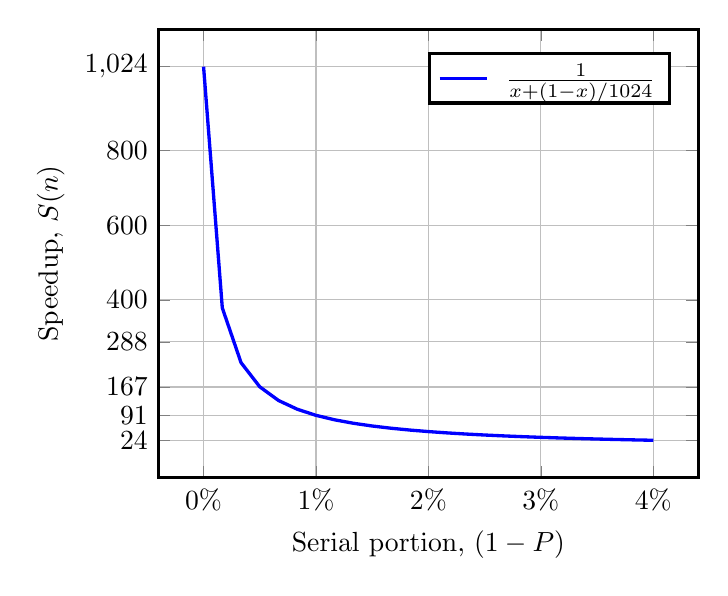
\begin{tikzpicture}
  \begin{axis}[
    ymajorgrids,
    xmajorgrids,
    ylabel={Speedup, $S(n)$},
    ytick={24,91,167,288,400,600,800,1024},
    xlabel={Serial portion, $(1-P)$},
    scaled x ticks = false, % do not add axis-multiplier
    xticklabel={% print percent
      \pgfmathparse{\tick*100}%
      \pgfmathprintnumber{\pgfmathresult}%
      \%%
    },
    legend style={
      at={(0.95,0.95)},
      anchor=north east,
      column sep=1ex
     },
     no markers,
     very thick
  ]

  \addplot+[domain=0.00:0.04] {1/(x+((1-x)/1024))};
  \addlegendentry{$\frac{1}{x + (1-x) / 1024}$};
  \end{axis}
\end{tikzpicture}
